% Outline:
% Overview
% Confounding description
% Latent Variable (and how to model them)
% Deconfounder description
% Deconfounder case study
% Alternatives
\section{Latent Confounding}
\label{sec:latent-confounding}

This section focuses on latent confounding in causal inference problems.
As mentioned in Section \ref{sec:graph-construction},  latent confounders affect the treatment assignment of our causal variables of interest, as well as the outcome.
While more complicated, this setup is the more realistic and typical case faced by demand modelers.
We first go over a few examples of confounding in transportation analyses and explain
the challenges that come with such cases.
Next we will briefly review a few approaches to dealing with latent confounding.

Then we focus specifically the recent de-confounder technique of \citet{wang_2019_blessings}.
In particular, we conduct a case study and simulation using the deconfounder.
Using data from \citet{brathwaite_asymmetric}, our case study shows how directed acyclic graphs can help clarify
one's reasoning regarding the number of confounders,
the assumptions for which variables are confounded,
and the models needed to estimate the causal effects.
Additionally, we use a simplified simulation scenario to investigate the usefulness
and pitfalls of the deconfounder approach for generating accurate model estimates.

\subsection{Examples of confounding}
\label{sec:confounding-examples}

Confounding occurs when a certain (confounding) variable induces variations in
both the outcome as well as the treatment (policy) variables of interest,
creating correlation between the treatment and the outcome that is not caused
by the treatment variable itself. When the confounding variable (or variables) is
observed, we can control for the confounding effect, and there exists many
methods in the literature for how to do that, including post-stratification,
multiple regression, propensity score methods, g-computation, targeted maximum likelihood estimation, etc.
It is when the confounding variable is unobserved that the problem becomes significantly more challenging.

For an illustration, imagine we're interested in the effect of adding a bike lane on the mode share of bicycling in a given neighborhood.
To estimate this effect, we might develop a disaggregate mode choice model with a dummy variable for whether a bike lane exists between an individual's trip origin and destination.
We might then wish to treat the coefficient on this variable as the causal effect of adding a bike lane on the log-odds of choosing to bike.
The problem with this strategy is that individuals may self-select to live in an area where bicycle infrastructure exists because they have a preference for commuting by bike.
In other words, if we define an additional variable to encode a person's latent, inherent preference for biking, then this variable determines both a person's likelihood for living in an area with existing bicycle infrastructure and whether that person chooses to bike.
This latent variable is subsequently expected to lack ``balance'' across the treatment and control groups: those who live near a bicycle lane are expected to have higher preference for biking than those who don't.
Accordingly, if we neglect the latent confounder as a source of variation in both our treatment and outcome variables,
then we risk biasing our treatment effect estimates of interest.

\subsection{Latent Variables}
\label{sec:latent-variables}
Latent confounders are a special case of latent variables, i.e. unobserved variables.
These include both psychological constructs and physically missing observations.
Psychological constructs include measurements about
happiness, lifestyle, economic expectation, morale, among many others.
Physically missing observations include measurement errors
(such as inexact measurements of key variables, data entry errors, or measurement inaccuracy),
missing data, survey item non-response, etc.

To cope with these latent variables, modelers make parameterized assumptions about how the latent variables relate to the observed variables.
Then, these parameters are inferred alongside the latent variables and used to estimate causal effects of interventions.
% ICLV is spelled out since readers may not remember from section 3.
Examples of such latent variable models include Integrated Choice and Latent Variable (ICLV), Generalized Linear Latent and Mixed Models (GLMM; including mixed logit models), Factor Analysis Models, and Latent Class Models.
For specific examples of these models being used to address latent confounding, see \citet{louizos_2017_causal} and \citet{perrakis_2019_latent} for factor analysis and latent class modeling examples, respectively.

From a choice modeling perspective, recall from Section \ref{sec:choice-graphs} that ICLV models have been used for decades.
The same is true of GLMMs / mixed-logit models.
These models address primarily address issues of latent mediation.
For mixed logit models this is evident in specifications where observable variables such as socio-demographics (e.g. income) cause an unobservable preferences (e.g. price sensitivity) that then influences the choice.
For ICLVs, recall Figure \ref{fig:example-graph-iclv} in Section \ref{sec:choice-graphs}.
Despite their primary focus on mediation, these models dovetail with latent confounding in the following instances.

Consider socio-demographic variables such as age.
Age may be thought to influence a latent attitude of environmental friendliness.
This latent attitude may then influence both whether one lives near bicycle infrastructure and what travel mode one chooses.
In this case, the latent variable of environmental friendliness is a latent mediator of age and the travel choice.
Simultaneously, the latent variable is a latent confounder of bicycle infrastructure presence and travel choice.

Here, failing to account for the latent attitudes may bias our observational study
if we're interested in the effect on bicycle mode share from adding a bike lane.
However, we could use an ICLV model to both address latent mediation and latent confounding.
For estimation, ICLV models usually rely on collecting indicator/proxy data to infer the levels of latent variable for individuals in a certain sample.
Unfortunately, the collection of this data is not always easy or even feasible.
For example, there may be sensitivity of individuals towards some attitudinal questions, or we may not be able to reach the individuals to conduct additional surveys with them.
This makes it difficult for researchers to collect necessary information that allows for controlling for unobserved confounders in models.

\subsection{The deconfounder algorithm}
\label{sec:deconfounder-algo}

One recent method that has been proposed to deal with the problem of latent
confounding without the need to collect additional data is the deconfounder
algorithm by \citet{wang_2019_blessings}. The method attempts to control for the
confounding variable by estimating a ``substitute confounder'': a set of variables
that once controlled for, renders all variation in the treatment variables of
interest exogenous. The process of applying the method can be stated simply.
It proceeds as follows:
\begin{itemize}
	\item First, estimate the substitute confounder using any good latent variable
	model the modeler chooses. The authors suggest estimating a factor model
	with k factors on the set of covariates the modeler is interested in.
	\item Second, check the factor model's accuracy using posterior predictive
	checks.
	\item Once a sufficiently accurate latent variable model is recovered, use it
	to estimate an expected value of the latent variable for each observation,
	and control for this value in the outcome model, alongside the treatment
	variables and other covariates of interest.
\end{itemize}



One main assumption of the deconfounder algorithm is that the data at hand
should only have multi-cause confounders, thus the title of the paper, ``The
blessings of multiple causes.'' In other words, this method works when all
unobserved confounders affect multiple of the observed causes (or treatment
variables) of interest, alongside the outcome. This assumption is weaker than
the standard ignorability assumption, which requires the absence of both
single cause and multi-cause confounders for accurate causal inferences.



\subsection{Case study: Simulation}
\label{sec:deconfounder-simulation}

The purpose of this section is to investigate the effectiveness of the
deconfounder algorithm \citep{wang_2019_blessings} in adjusting for unobserved
confounding. We use simulated mode choice data where travel distance
linearly confounds both travel time and travel cost. We then mask the travel
distance data and treat it as an unobserved variable.


We estimate three models:

\begin{itemize}
	\item Model 1: A multinomial logit with the correct original specification,
	except we omit the travel distance variable in the specification without
	trying to adjust for it. This model represents the worst case scenario
	where a modeler ignores, or is unaware of, unobserved confounding.
	\item Model 2: We use the deconfounder algorithm to try to recover the
	confounder (travel distance). In this method, we use all the variables in
	each mode's utility to recover that mode's confounder. This is in line
	with the approach taken in \citet{wang_2019_blessings}, where they use all the
	of observed variables in the factor model to recover a substitute
	confounder.
	\item Model 3: We use the deconfounder algorithm to try to recover the
	confounder (travel distance), but this time, we only use travel time and
	cost in the factor model, instead of all the variables in the utility
	specification of each mode. By only using what we know are confounded
	variables to recover the substitute confounder, our goal is to analyze
	whether we can improve the accuracy of this approach by adopting a stronger
	prior on which variables are confounded. This can
	be in the form of building and testing candidate causal graphs that
	try to illustrate this confounding.
\end{itemize}


We compare both the coefficient estimates on travel time and cost from
each of those three models to the true estimates used in the simulation.
We also compare the distribution of the recovered substitute confounder under each of
models 2 and 3 to the true confounder. The main findings of this exercise are the following:


Using the true variables believed to be confounded (i.e. method 3 where only
travel time and cost are used to recover the confounder) leads to a better
recovery of the true confounder. Figure \ref{fig:qq-plot-method-2} and \ref{fig:qq-plot-method-3} show a QQ plot of the true
and recovered confounders under models 2 and 3 respectively. Looking at those
figures, we see that the distribution of the recovered substitute
confounder under method 3 is closer to that of the true confounder than method
2. This suggests that it may be better to run the deconfounder algorithm based
on a hypothesized causal graph, rather than just running it on all the
observed covariates. Please refer to Section \ref{sec:graph-construction} for how to build plausible causal graphs.


\begin{figure}
   \centering
   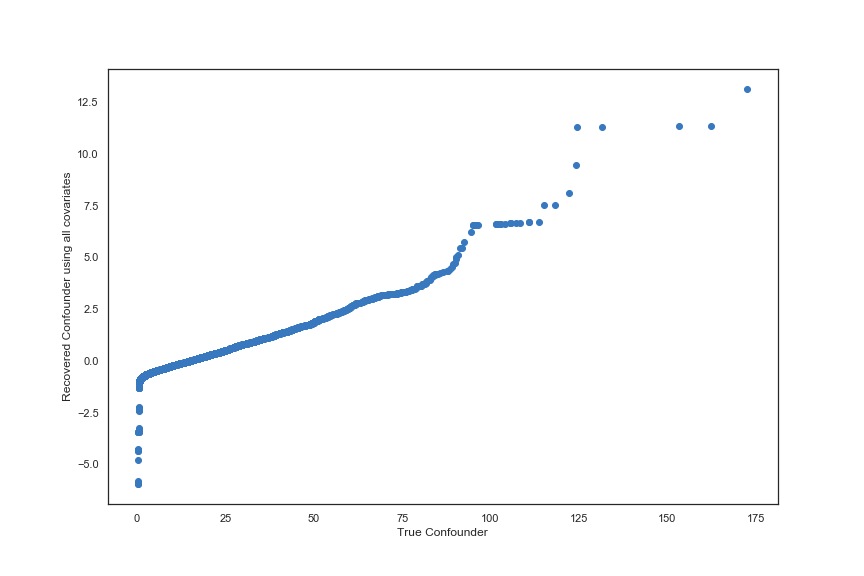
\includegraphics[width=0.5\textwidth]{qq-plot-method-2.png}
   \caption{QQ plot of true confounder against recovered confounder using all covariates}
   \label{fig:qq-plot-method-2}
\end{figure}

\begin{figure}
   \centering
   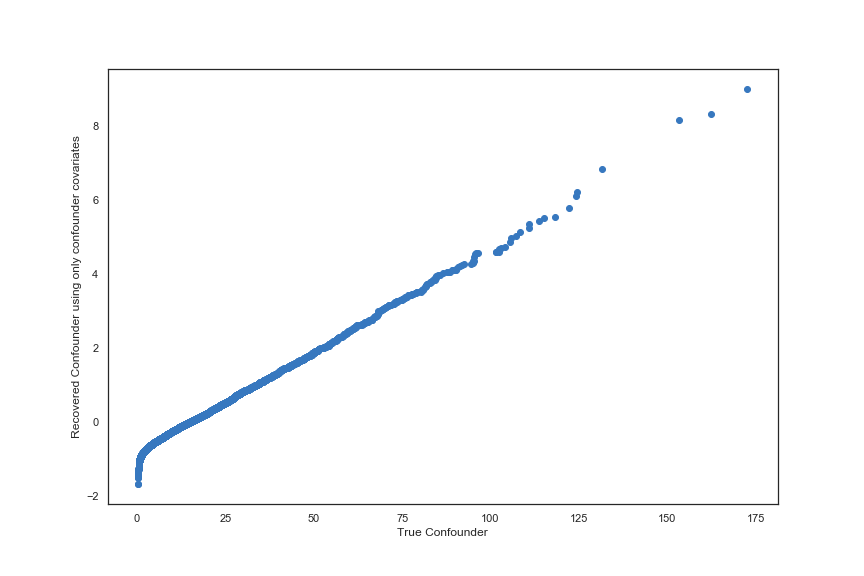
\includegraphics[width=0.5\textwidth]{qq-plot-method-3.png}
   \caption{QQ plot of true confounder against recovered confounder using all covariates}
   \label{fig:qq-plot-method-3}
\end{figure}


Additionally, and perhaps most importantly, the effectiveness of the
deconfounder algorithm is very sensitive to small errors and misfits in the
recovered confounder.
This can be seen in three ways.
First, although method 3 returns a relatively good fit of the
true confounder (based on the QQ plot), the adjusted coefficients on travel
time and cost do not exhibit any reduction in the bias resulting from
omitting the true confounder.
Second, the time and cost coefficient estimates
recovered using the actual confounder values are outside of confidence intervals
of the estimates using any of models 1, 2, or 3.
The deconfounder-powered estimates are certain in their incorrectness.
Third, the coefficients on the recovered confounder are highly insignificant.
This raises questions about the usefulness of the deconfounder algorithm in practice.

Limitations notwithstanding, it is
important to point out that sensitivity to small errors and misfits is not only a by-product of the deconfounder
algorithm itself. In fact, it is one of the built in characteristic of omitted
variable bias, and perhaps more broadly, the problem of error-in-variables in
regression. To illustrate this, suppose we actually observe the true
confounder variable, but with some white, random Gaussian noise. Figure \ref{fig:confounder-sensitivity}
shows how the bias in the parameter of interest increases quickly as a
function of the standard deviation of the random noise. This emphasizes the
difficulty of recovering unbiased estimates in the presence latent confounders,
and highlights potential limitations with methods that attempt to recover a
substitute confounder to control for.

\begin{figure}
   \centering
   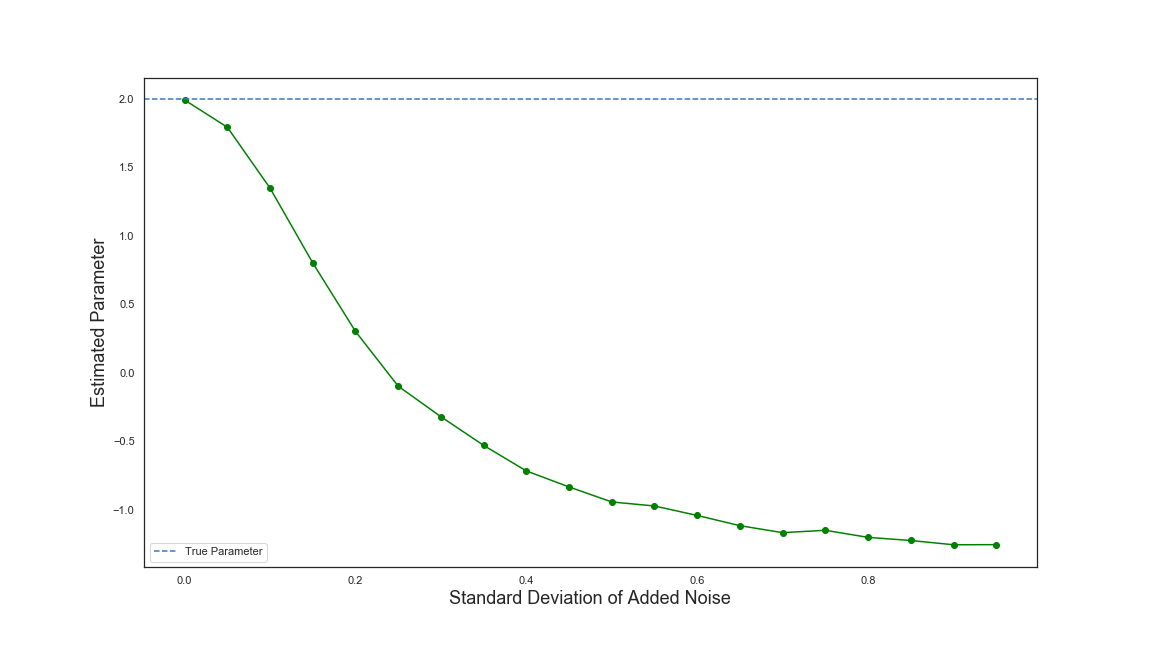
\includegraphics[width=0.5\textwidth]{confounder-sensitivity.png}
   \caption{Sensitivity of causal estimates to random errors in the confounder variable}
   \label{fig:confounder-sensitivity}
\end{figure}

\subsection{Alternatives}
\label{sec:deconfounder-alternatives}
Given the algorithmic difficulties with accurately inferring latent confounders,
we encourage analysts to investigate and experiment with alternative methods of
coping with unobserved confounding.
In particular, we advise researchers to conduct sensitivity analyses and to compute bounds for their treatment effects of interest.
Sensitivity analyses estimate the strength of relationship between a latent confounder and one's treatment variables that is needed to invalidate one's results.
Audiences are then able to judge whether it is plausible for a confounder of that strength to exist.
For more information about and demonstration of this technique for dealing with latent confounding,
see \citet{rosenbaum_1983_assessing}, \citet{liu_2013_introduction}, and \citet{jung_2020_bayesian}.
For related literature and guidance on bounding one's treatment effects in the presence of latent confounding,
see \citet{manski_1990_nonparametric}, \citet{richardson_2014_nonparametric}, and \citet{geiger_2014_estimating}.
The crux of this research is that even with unobserved confounding, we can derive credible bounds for our treatment effects.
This enables us to avoid the difficulties of trying to provide accurate point estimates via accurate reconstruction of the latent confounders.
